\documentclass[a4paper,12pt]{article}
\usepackage[utf8]{inputenc}
\usepackage[english,russian]{babel}
\usepackage[T2A]{fontenc}
\usepackage{mathtext}
\usepackage{gauss}
\usepackage{graphicx}
\usepackage{amsmath, amsfonts, amssymb}
\newtheorem{theorem}{Теорема}
\usepackage[left=2.50cm, right=2.00cm, top=2.00cm, bottom=2.00cm]{geometry} 
\usepackage{mathdots} 
\usepackage[pdftex]{lscape}
\usepackage{mathtools}
\usepackage{pgfplots}
\pgfplotsset{compat=1.9}
\usepackage{graphicx}%Вставка картинок правильная
\usepackage{tikz}
\usepackage{float}%"Плавающие" картинки
 \usepackage{relsize}
\usepackage{wrapfig}%Обтекание фигур (таблиц, картинок и прочего)
\usepackage{ tipa }
\usepackage{amsmath}
  \usepackage[unicode=true, colorlinks=true, linkcolor=blue, urlcolor=blue]{hyperref}
\linespread{1}
\newcommand{\om}{\overline{o}}
\newcommand{\OB}{\underline{O}}
\newcommand{\eps}{\varepsilon}
\newcommand{\RR}{\mathbb{R}}
\newcommand{\NN}{\mathbb{N}}
\newcommand{\CC}{\mathbb{C}}
\newcommand{\QQ}{\mathbb{Q}}
\newcommand{\ZZ}{\mathbb{Z}}
\newcommand{\dx}{\d{dx}}
\newcommand{\ph}{\varphi}
\newcommand{\F}{\mathbb{F}}
\newcommand{\E}{\mathbb{E}}
\begin{document}
    \section*{1}{
    $$f(x) =\frac{3x-7}{(x^2-1)^2}$$
    $$f^{'}(x) = \frac{-(9x-1)(x-3)}{(x^2-1)^3}  $$
    $$\text{Точки }-\frac19, 3, -1,1 - \text{точки экстремума}$$
    \begin{figure}[h]
    	
    	\centering
    	
    	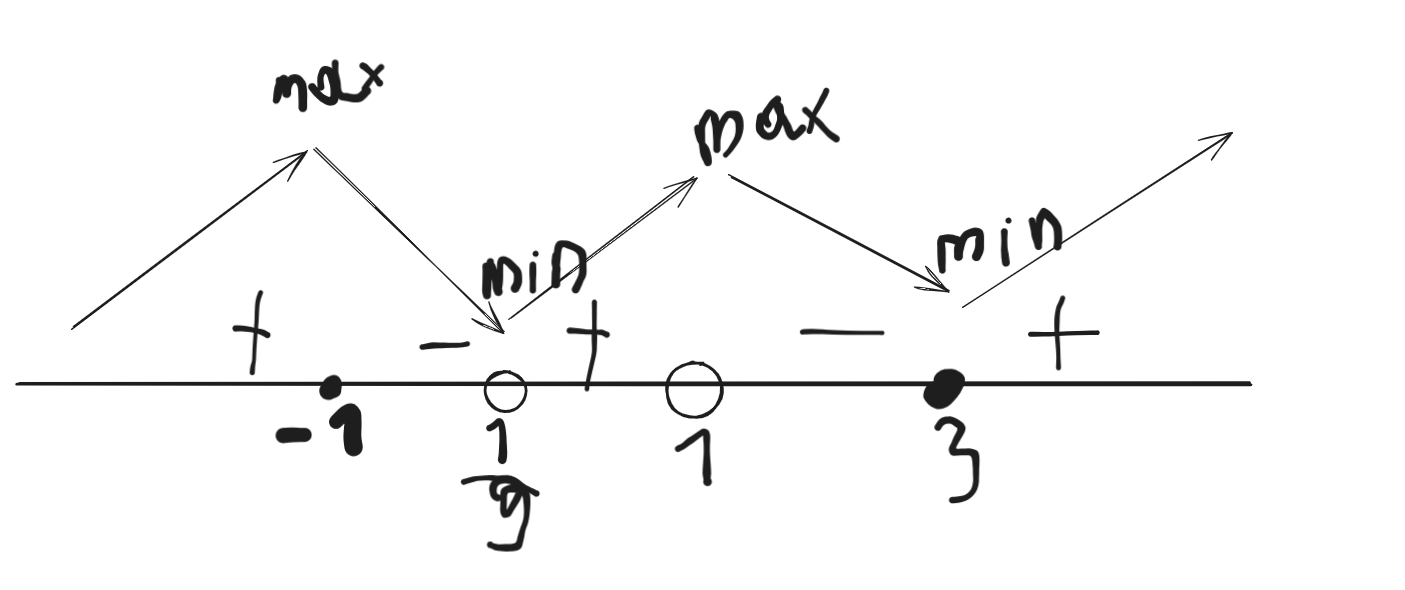
\includegraphics[width=0.8\linewidth]{Screenshot from 2024-01-15 20-13-23.png}
    	
    	\caption{Точки экстремумов}
    	
    	\label{fig:mpr}
    	
    \end{figure}
$$f(\frac19) = -\frac{2187}{320}$$
$$f(3) = \frac{5}{16}$$
3 - точка глобального максимума. Глобального максимума нет.
\subsection*{2)}
$$f(x) = \begin{cases*}x^{x\ln x}, x>0 \\
   1, x = 0\end{cases*}$$
   $(x^{x\ln x})^{'} = (e^{x\ln^2x})^{'} = x^{x\ln x}\cdot(2\ln x + \ln^2x ) $\\
   $f^{'}(0) = \lim_{h\to 0}\frac{f(0+h-f(0))}{h} = \lim_{h\to0} \frac{h^{h\ln h}-1}{h} \nexists$
   $$f^{'}(x) = \begin{cases*}
 (x^{x\ln x})^{'} = (e^{x\ln^2x})^{'} = x^{x\ln x}\cdot(2\ln x + \ln^2x ) , \quad x>0
   \end{cases*}$$
   $$x^{x\ln x}\cdot(2\ln x + \ln^2x ) = 0$$
   $$x = 1 || x = \frac{1}{e^2}$$
       \begin{figure}[h]
   	
   	\centering
   	
   	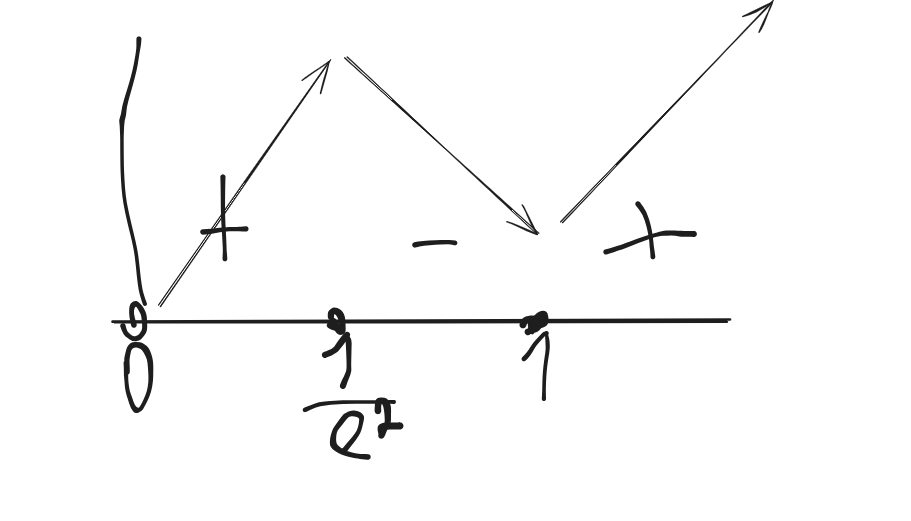
\includegraphics[width=0.8\linewidth]{Screenshot from 2024-01-15 20-35-33.png}
   	\caption{Точки экстремумов}
   	\label{fig:mpr}
   \end{figure}
   $$f(1) = 1$$
   1 и 0 точки глобальных минимумов
   \section*{2}
    $$f(x) =\begin{cases}
   	\sin x , x\geqslant 0 \\
   	x^2 , x< 0
   \end{cases}$$
    $$f^{'}(x) = \begin{cases}
   		\cos x, x\geqslant 0 \\
   		2x , x<0
   \end{cases}$$
   $\cos x =0 \iff x = \frac{\pi}{2}+\pi n $ - точки экстремум. 
   Чтобы узнать, когда функция выпуклая возьмем вторую производную и узнаем знаки функции в точках экстремум. 
          \begin{figure}[h]
   	
   	\centering
   	
   	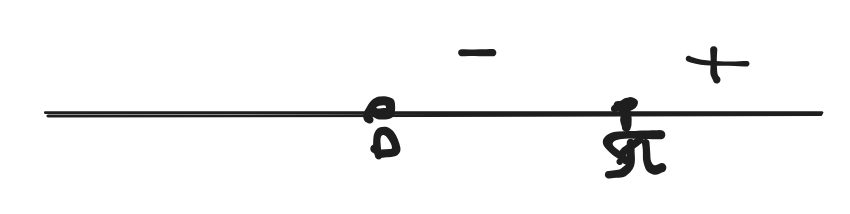
\includegraphics[width=0.8\linewidth]{Screenshot from 2024-01-15 20-53-03.png}
   	\caption{}
   	\label{fig:mpr}
   	$$\text{на интервалах вида } (2n\pi; (2n+1)\pi)\text{ функция выпукла}$$
   	   	$$\text{на интервалах вида } ((2n+1)\pi; 2n\pi)\text{ функция вогнута}$$
   	
   \end{figure}
    \section*{3 }
    \subsection*{a)}
    $$1+\frac{x}{2}-\frac{x^2}{8}<\sqrt{1+x}< 1+\frac{x^2}{2}$$
    $$\sqrt{1+x} = 1+\frac{x}{2}-\frac{x^2}{8} + R_n(x)$$
	$$1+\frac{x}{2}-\frac{x^2}{8}<1+\frac{x}{2}-\frac{x^2}{8} + R_n(x)< 1+\frac{x^2}{2}$$ 
	%$$0 < R_n(x)<\frac{5x^2}{8}-\frac{x}{2}$$
	$$\begin{cases*}
		1+\frac{x}{2}-\frac{x^2}{8}<1+\frac{x}{2}-\frac{x^2}{8} + R_n(x) \\
		\frac{x}{2}-\frac{x^2}{8} + R_n(x)< \frac{x^2}{2}
	\end{cases*} $$
  Очевидно, что эти неравенства выполняются при любом положительном x
  \subsection*{b)}
  $$\frac{b-a}{b}< \ln{\frac{b}{a}}<\frac{b-a}{a}, 0<a<b$$
  \section*{4}
  \subsection*{a)}
  $$\text{Рассмотрим функцию}  f(t) = t^t- \text{ она выпуклая.}$$
   $$\pi^\pi=f\left(\frac{x+y+z}{3}\right)<\frac{f(x)+f(y)+f(z)}{3}$$
   $$108<3\pi^\pi <x^x+y^y+z^z$$
   \subsection*{b)}
   $$\frac{x_1+\dots + x_n}{n}\geqslant \sqrt[n]{x_1\dots x_n}$$
   $$\ln{\left(\frac{x_1+\dots + x_n}{n}\right)}\geqslant \frac{1}{n}\ln x_1 + \dots + \frac{1}{n}\ln x_n$$
   $$-\ln{\left(\frac{x_1+\dots + x_n}{n}\right)}\leqslant -\frac{1}{n}\ln x_1 + \dots + -\frac{1}{n}\ln x_n$$
   $$\text{Так как -lnx функция выпуклая, то для нее выполняется неравенство Йенсена}$$
   \section*{5}
   $$\sin\left(\frac{A+B+C}{3}\right)\leqslant \frac{\sin A + \sin B +\sin C}{3} $$
     $$3\sin\left(\frac{\pi}{3}\right)\leqslant \sin A + \sin B +\sin C $$
     $$\text{Равенство достигается. когда } A =B = C = \frac{pi}{3}$$
     $$\sin A + \sin B +\sin C  = \frac{3\sqrt3}{2}$$
 \end{document}
